\documentclass[11pt]{article}
\usepackage[margin=1in]{geometry}
\usepackage{amsmath,amssymb,amsthm,mathtools}
\usepackage{graphicx}
\usepackage{microtype}
\usepackage[hidelinks]{hyperref}
\newtheorem{theorem}{Theorem}
\newtheorem{lemma}[theorem]{Lemma}
\newtheorem{corollary}[theorem]{Corollary}
\newcommand{\Cu}{C_u^*}
\newcommand{\ellTwo}{\ell_2}
\newcommand{\SOT}{\mathop{\mathrm{SOT}\!-\!\sum}}
\title{Rank-two block projections contain block-rank-one projections}
\author{Automated Math Discovery Run \texttt{fa\_banach\_001}\\Model: GPT5.6}
\date{22 July 2026}
\begin{document}
\maketitle
\begin{center}
\fbox{\begin{minipage}{0.91\textwidth}
\textbf{Claimed status: partial result, subject to human review.}
The theorem fully answers the rank-two block-projection question, but not
Question~6.1 for arbitrary Boolean families of projections of rank greater
than one.
\end{minipage}}
\end{center}
\section{Source questions}
Braga, Farah, and Vignati ask in Question~6.1 whether a sequence of
projections $p_n\in\Cu(X)$ whose every strong subseries belongs to
$\Cu(X)$ admits rank-one subprojections with the same property
\cite[Question~6.1, p.~20]{BFV}. The exact source passage is reproduced below.
\begin{figure}[ht]
\centering

\includegraphics[width=0.95\textwidth]{figures/open_problem_crop.png}
\caption{Question~6.1 in the source paper.}
\end{figure}
The rank-two block case was restated as an explicit open question in
Vignati's 2026 habilitation \cite[Question~5.31, p.~53]{Vig}: if
$p=\SOT_n p_n$ is a noncompact block ghost projection and every $p_n$
has rank two, must there be rank-one $q_n\leq p_n$ such that
$\SOT_nq_n\in\Cu(X)$?
\begin{figure}[ht]
\centering
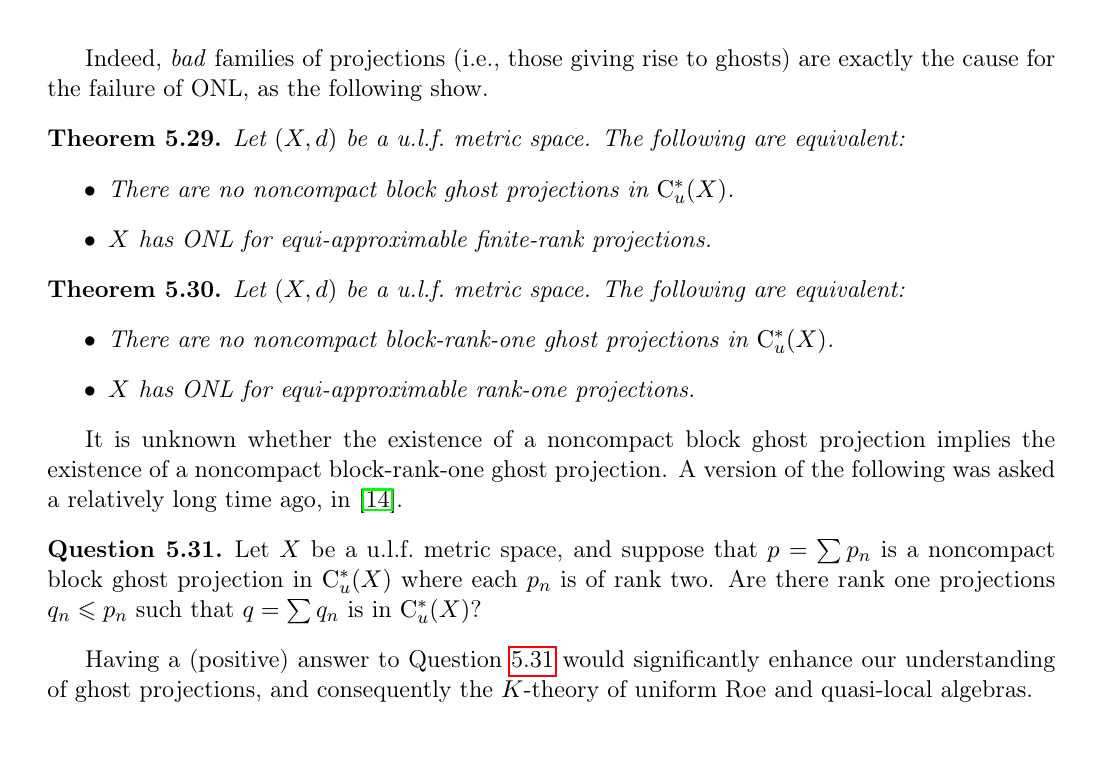
\includegraphics[width=0.94\textwidth]{figures/rank_two_question_crop.png}
\caption{The rank-two block question in the 2026 habilitation.}
\end{figure}
\clearpage
\section{Definitions and scope}
Let $X$ be a uniformly locally finite metric space. A projection
$p\in\Cu(X)$ is a \emph{block projection} if there are pairwise disjoint
finite sets $X_n\subseteq X$ such that
\[
 p=\SOT_{n\in\mathbb N}p_n,\qquad p_n=\chi_{X_n}p\chi_{X_n}.
\]
The $p_n$ are mutually orthogonal finite-rank projections. It is
\emph{block-rank-one} when every nonzero $p_n$ has rank one.
An operator $a\in\Cu(X)$ is a \emph{ghost} if its matrix coefficients
tend to zero at infinity. We use only two elementary facts: diagonal
multipliers $\chi_A$ lie in $\ell_\infty(X)\subseteq\Cu(X)$, and
$\Cu(X)$ is closed under continuous functional calculus.
\section{Proof intuition}
Inside a two-dimensional subspace, some coordinate cut always distinguishes
two orthogonal directions by a fixed amount. More precisely, for a suitable
subset $A_n\subseteq X_n$, the two eigenvalues of
$p_n\chi_{A_n}p_n$ are separated by at least $1/4$. There are then only
finitely many spectral thresholds needed to separate the larger eigenvalue
from the smaller one in every block. For each threshold class, continuous
functional calculus extracts the larger eigenspace simultaneously. Adding
the finitely many classes produces the desired block-rank-one projection.
\section{The diagonal-gap lemma}
\begin{lemma}[uniform two-dimensional coordinate gap]\label{lem:gap}
Let $E$ be a two-dimensional subspace of $\ellTwo(F)$, where $F$ is finite,
and let $P$ be the orthogonal projection onto $E$. There is $A\subseteq F$
such that the two eigenvalues of $(P\chi_A P)|_E$ differ by at least $1/4$.
\end{lemma}
\begin{proof}
Choose an orthonormal basis $u,v$ of $E$. For $x\in F$, put
\[
 d_x=|u(x)|^2-|v(x)|^2,\qquad z_x=\overline{u(x)}v(x).
\]
Then $\sum_xd_x=0$ and $\sum_xz_x=0$. For any $A\subseteq F$, the
eigenvalue gap of $(P\chi_A P)|_E$ is
\begin{equation}\label{eq:gap}
 \left(\left|\sum_{x\in A}d_x\right|^2+
 4\left|\sum_{x\in A}z_x\right|^2\right)^{1/2}.
\end{equation}
Set $D=\sum_x|d_x|$. If $D\geq 1/2$, take
$A=\{x:d_x\geq0\}$. Since $\sum_xd_x=0$,
$\sum_{x\in A}d_x=D/2\geq1/4$, and \eqref{eq:gap} gives the result.
Suppose $D<1/2$. Writing $a_x=|u(x)|^2$ and $b_x=|v(x)|^2$, we have
\[
 2|z_x|=2\sqrt{a_xb_x}\geq a_x+b_x-|a_x-b_x|.
\]
Thus $L:=\sum_x|z_x|>(2-1/2)/2=3/4$. Averaging over
$\theta\in[0,2\pi]$ gives a $\theta$ such that
\[
 \sum_x\left|\operatorname{Re}(e^{-i\theta}z_x)\right|\geq\frac{2L}{\pi}.
\]
Let $A=\{x:\operatorname{Re}(e^{-i\theta}z_x)\geq0\}$. Because
$\sum_xz_x=0$,
\[
 \left|\sum_{x\in A}z_x\right|\geq\frac{L}{\pi}>\frac{3}{4\pi}.
\]
The second term in \eqref{eq:gap} makes the gap larger than
$3/(2\pi)>1/4$.
\end{proof}
\section{Rank-two block selection}
\begin{theorem}\label{thm:main}
Let $X$ be a uniformly locally finite metric space and let
$p\in\Cu(X)$ be a block projection with respect to pairwise disjoint
finite sets $(X_n)_{n\in\mathbb N}$. Suppose every nonzero block
$p_n=\chi_{X_n}p\chi_{X_n}$ has rank two. Then there are rank-one
projections $q_n\leq p_n$ such that
\[
 q=\SOT_{n\in\mathbb N}q_n\in\Cu(X).
\]
In fact, for every $M\subseteq\mathbb N$,
$q_M=\SOT_{n\in M}q_n$ belongs to $\Cu(X)$.
\end{theorem}
\begin{proof}
By Lemma~\ref{lem:gap}, for every $n$ there is $A_n\subseteq X_n$ such
that the two eigenvalues
\[
0\leq\lambda_n^-\leq\lambda_n^+\leq1
\quad\text{of}\quad h_n=(p_n\chi_{A_n}p_n)|_{p_n\ellTwo(X)}
\]
satisfy $\lambda_n^+-\lambda_n^-\geq1/4$.
Let $T=\{k/16:1\leq k\leq15\}$. For every $n$, choose
$t(n)\in T$ so that
\begin{equation}\label{eq:margin}
\lambda_n^-+\frac1{32}\leq t(n)\leq\lambda_n^+-\frac1{32}.
\end{equation}
Such a grid point exists because the interval between the two endpoints has
length at least $3/16$. Put $I_t=\{n:t(n)=t\}$ and $A=\bigcup_nA_n$.
For $I\subseteq\mathbb N$, set
\[
p_I=\SOT_{n\in I}p_n
=\chi_{\bigcup_{n\in I}X_n}p\chi_{\bigcup_{n\in I}X_n}.
\]
Hence $p_I\in\Cu(X)$. For every $t\in T$,
\[
a_t=p_{I_t}\chi_Ap_{I_t}
=\SOT_{n\in I_t}p_n\chi_{A_n}p_n
\]
also belongs to $\Cu(X)$. Choose a continuous function
$f_t:[0,1]\to[0,1]$ that is zero on $[0,t-1/64]$ and one on
$[t+1/64,1]$. The margins in \eqref{eq:margin} imply that
\[
q^{(t)}:=f_t(a_t)
\]
is the block projection whose block in $p_n\ellTwo(X)$, for $n\in I_t$,
is the spectral projection of $h_n$ associated with $\lambda_n^+$.
Thus every nonzero block of $q^{(t)}$ has rank one, and continuous
functional calculus gives $q^{(t)}\in\Cu(X)$.
Since $T$ is finite,
\[
q=\sum_{t\in T}q^{(t)}\in\Cu(X).
\]
Writing $q_n=\chi_{X_n}q\chi_{X_n}$ yields rank-one $q_n\leq p_n$ and
$q=\SOT_nq_n$. Finally, for every $M\subseteq\mathbb N$,
\[
q_M=\chi_{\bigcup_{n\in M}X_n}q\chi_{\bigcup_{n\in M}X_n}\in\Cu(X).
\]
\end{proof}
\begin{corollary}\label{cor:ghost}
Every noncompact block ghost projection in $\Cu(X)$ whose blocks have
rank two contains a noncompact block-rank-one ghost projection.
Consequently, Question~5.31 of \cite{Vig} has an affirmative answer.
\end{corollary}
\begin{proof}
Apply Theorem~\ref{thm:main}. The resulting $q$ has infinite rank and is
therefore noncompact. Since $0\leq q\leq p$, for every $x,y\in X$,
\[
|\langle q\delta_y,\delta_x\rangle|^2
\leq\langle q\delta_x,\delta_x\rangle\langle q\delta_y,\delta_y\rangle
\leq\langle p\delta_x,\delta_x\rangle\langle p\delta_y,\delta_y\rangle.
\]
The diagonal of the ghost projection $p$ vanishes at infinity, so the
display shows that $q$ is a ghost.
\end{proof}
\section{Verification, limitations, and novelty}
The script \texttt{code/verify\_rank\_two\_gap.py} numerically enumerates
all coordinate subsets for random finite rank-two subspaces and checks the
$1/4$ gap bound. This is only a consistency check; Lemma~\ref{lem:gap} is
the proof.
The result does not settle Question~6.1 for arbitrary families, nor does it
show that every higher-rank block ghost projection contains a rank-two block
ghost subprojection. It removes the complete rank-two block obstruction.
A bounded search on 22 July 2026 covered arXiv, the published EMS version,
exact phrases from Question~6.1, combinations of uniform Roe, rank two, and
rank-one subprojection, and Vignati's January 2026 habilitation. No prior proof
of this rank-two selection statement was found; the habilitation still labels
it Question~5.31. This is not an exhaustive novelty claim. Human review should
focus on the finite-threshold functional calculus step and the ghost
domination argument.
\begin{thebibliography}{9}
\bibitem{BFV}
B. M. Braga, I. Farah, and A. Vignati,
\emph{Operator norm localization property for equi-approximable families
of projections}, J. Noncommut. Geom. 18 (2024), no. 2, 657--680;
arXiv:2211.02775, DOI:
\href{https://doi.org/10.4171/JNCG/555}{10.4171/JNCG/555}.
\bibitem{Vig}
A. Vignati, \emph{Rigidity of Roe-like algebras},
M\'emoire d'habilitation \`a diriger des recherches, 2026,
Question~5.31, p.~53.
\end{thebibliography}
\end{document}
